\subsection{Rad-Graphen}
Der vorletzte Stop auf unserer Reise sind die sogenannten Wheel-Graphen. Hier wird zu einem zyklischen Graphen $C_n$ mit Knoten $\{v_1,..,v_n\}$, $n \geq 3$ ein weiterer Knoten $z$ hinzugefügt, der mit allen anderen Knoten benachbart ist, sodass der Wheel-Graph $W_{n}$ entsteht (Achtung: $W_n$ hat $n+1$ Knoten).
\begin{Tm}
Für die Anzahl der Spannbäume in einem Rad gilt:
\begin{equation}
 \mathit{k}\left(W_n\right) = \left(\frac{3+\sqrt{5}}{2}\right)^n+\left(\frac{3+\sqrt{5}}{2}\right)^n-2
 \label{wn}
\end{equation}
\end{Tm}
\textbf{Beweis:}\\
Um die Formel für die Berechnung der Anzahl der Spannbäume eines solchen Graphen herzuleiten, lassen wir von ~\cite{sedlacek_1970} inspirieren.
Wir beobachten, dass wir den Fan-Graphen $F_n$ bekommen, wenn wir die Kante $v_1v_n$ aus $W_n$ entfernen.
Die Anzahl der Spannbäume von $F_n$ kennen wir bereits von oben.
Um die Anzahl der Spannbäume von Rädern zu berechnen, zeigen wir zuerst die rekursive Beziehung
\begin{equation}
 \mathit{k}\left(W_{n+1}\right) = \mathit{k}\left(F_{n+1}\right) + \mathit{k}\left(F_n\right) + \mathit{k}\left(W_n\right)
\end{equation}
Um das zu tun, werden die Spannbäume von $W_{n+1}$ in drei verschiedene Klassen einteilen:\\
\par
\begingroup
\leftskip=20pt
\rightskip=20pt
\noindent
\textbf{1)} Alle Spannbäume, die die Kante $v_{n+1}v_1$, aber nicht die Kante $v_{n+1}z$ enthalten; das sind genau so viele, wie die Spannbäume von $W_n$, wie man in der Abbildung~\ref{klasse1} sehen kann. Wir beachten hier, dass ein $W_n$ entsteht, wenn man im $F_n$ eine Kante zwischen den beiden Knoten mit Grad $2$ hinzufügt.\\
\textbf{2)} Alle Spannbäume, die die Kante $v_{n+1}v_1$ nicht enthalten; das sind genau so viele, wie die Spannbäume von $F_{n+1}$; das wird aus Abbildung~\ref{klasse2} ersichtlich\\
\textbf{3)} Alle Spannbäume, die die Kante $v_{n+1}v_1$ und die Kante $v_{n+1}z$ enthalten; Wir beweisen gleich, dass das so viele sind, wie die Spannbäume von $F_n$.\\
\par
\endgroup
%\begin{figure}[h]
    \begin{minipage}{0.45\textwidth}
        \centering
        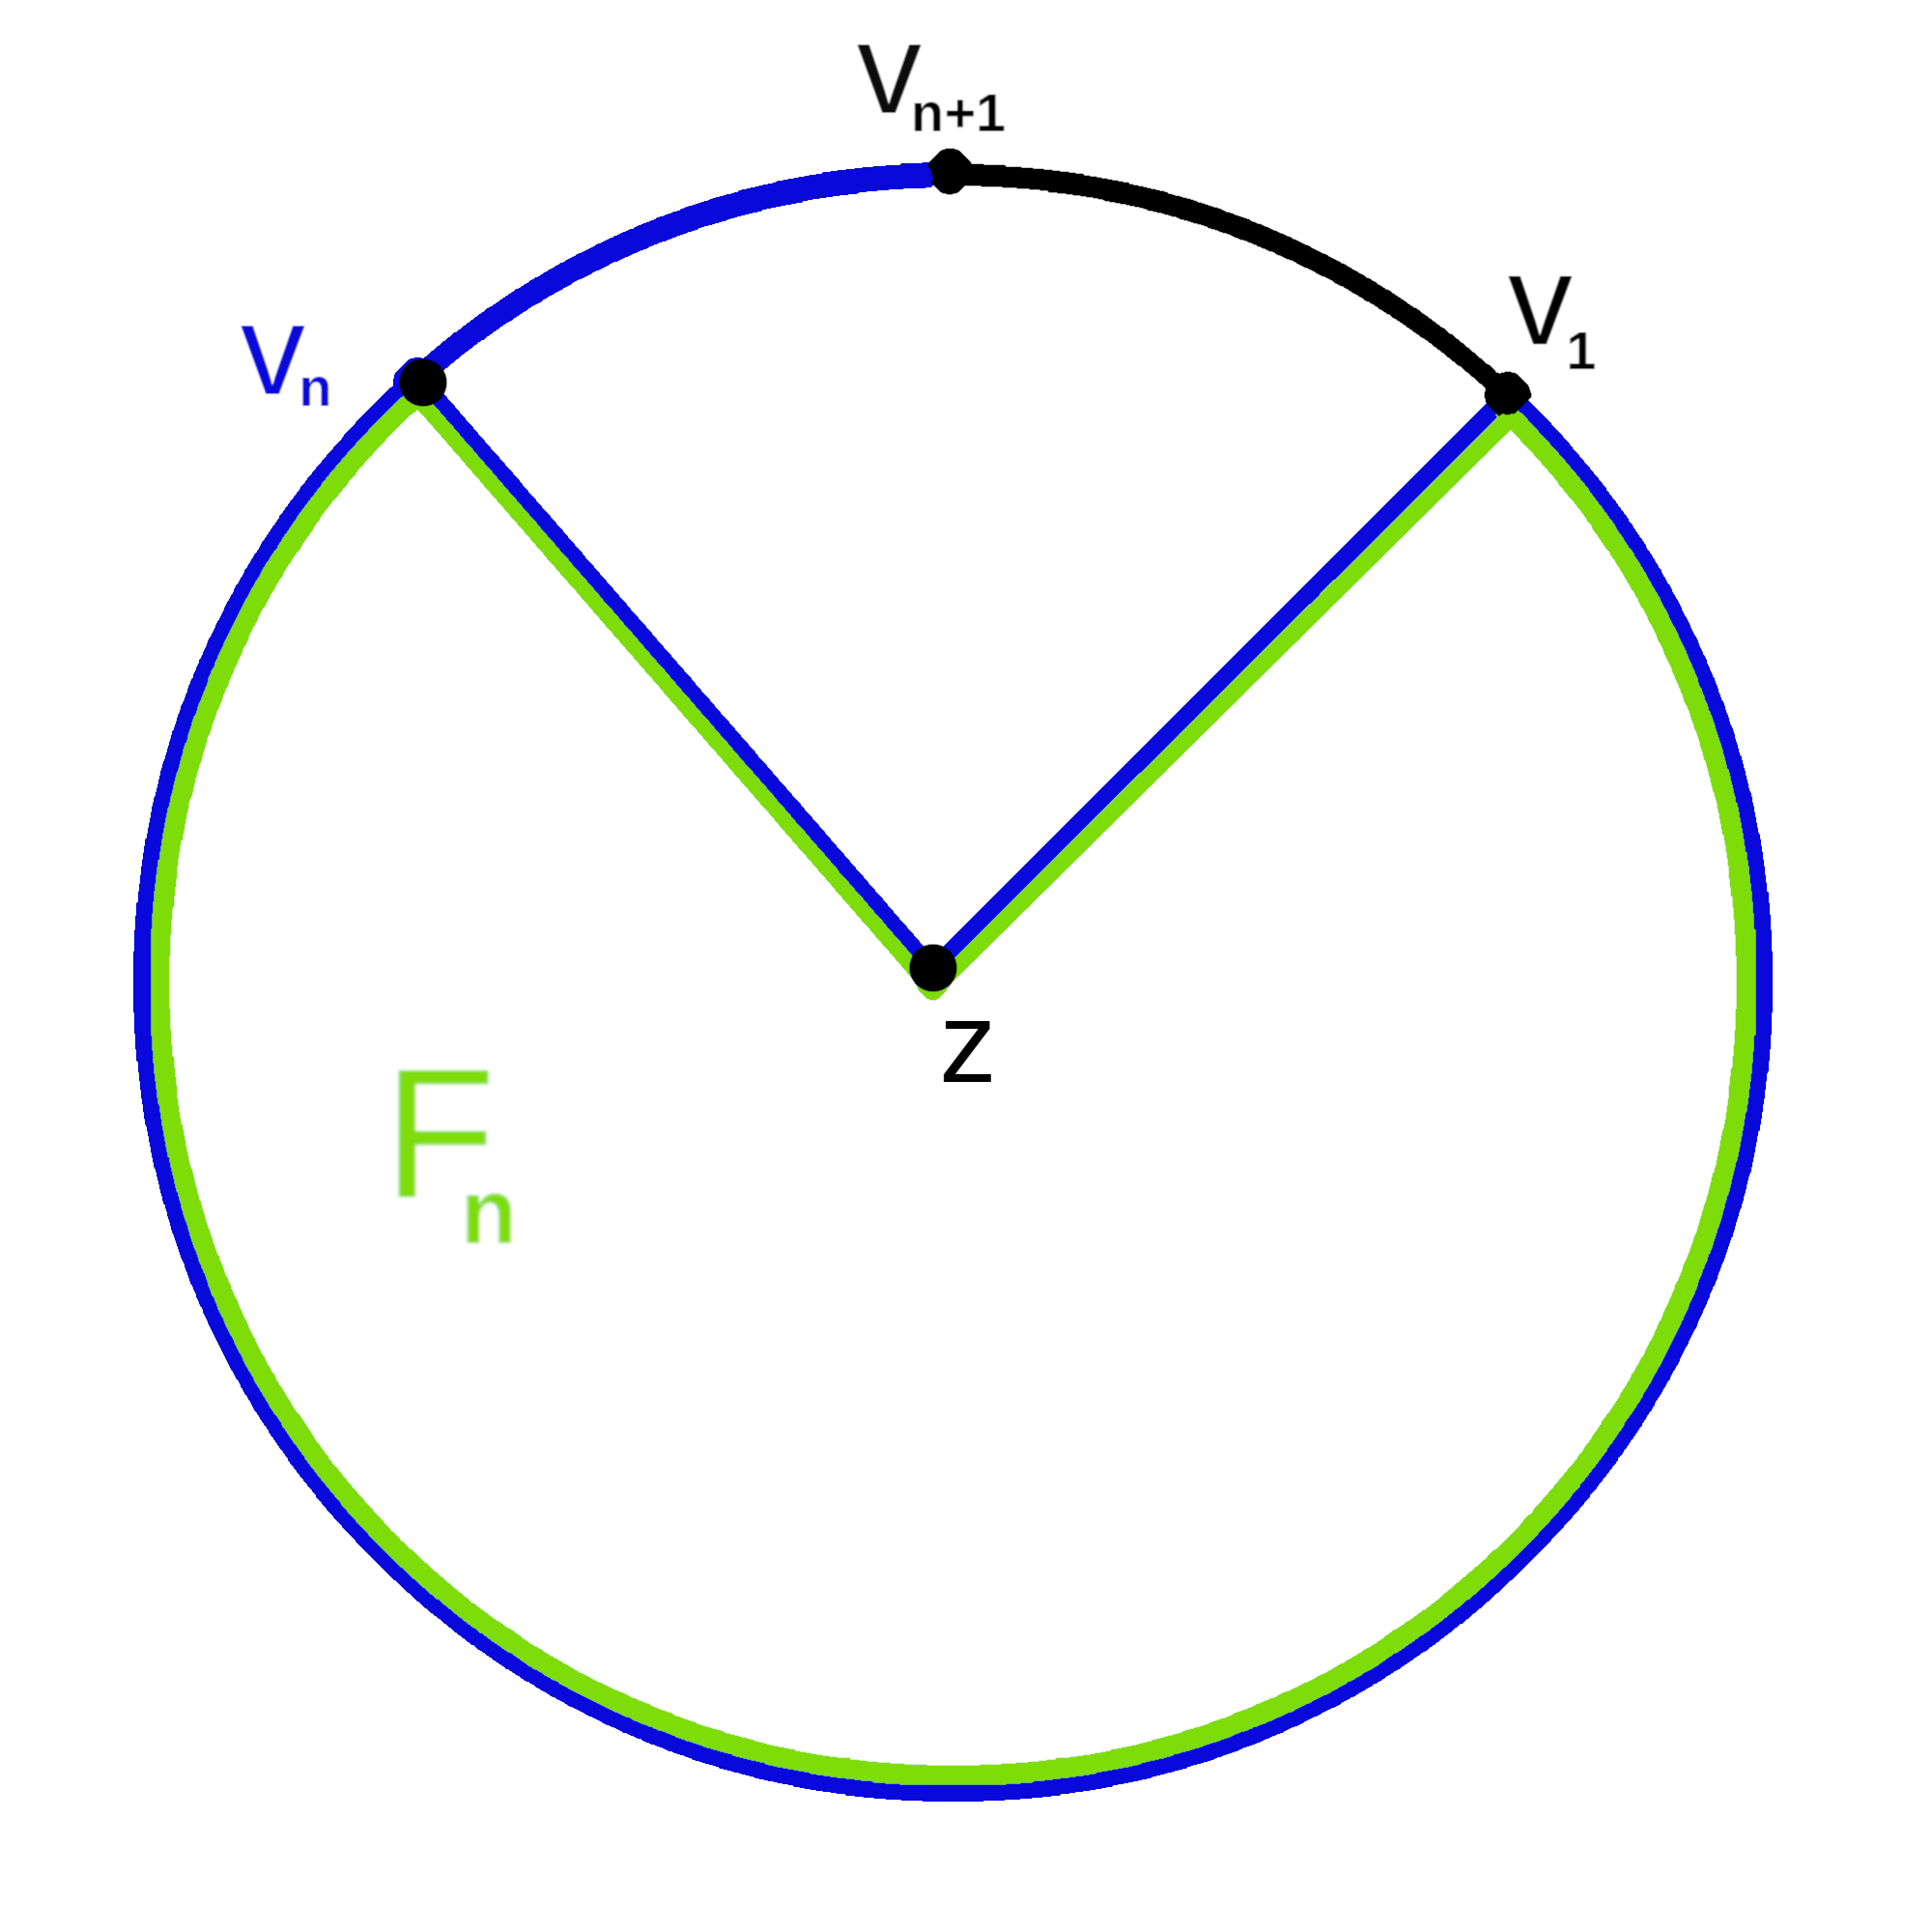
\includegraphics[width=1\textwidth]{klasse11.png}
        %\caption{In Klasse 1 sind die Spannbäume dieses Graphen, wobei die schwarze Kante in diesen Spannbäumen enthalten sein muss und der grün markierte Teil ein $F_n$ ist.}
        \captionof{figure}{In Klasse 1 sind die Spannbäume dieses Graphen, wobei die schwarze Kante in diesen Spannbäumen enthalten sein muss und der grün markierte Teil ein $F_n$ ist.}
 \label{klasse1} %caption vor label unbedingt
    \end{minipage}\hfill
    \begin{minipage}{0.45\textwidth}
        \centering
        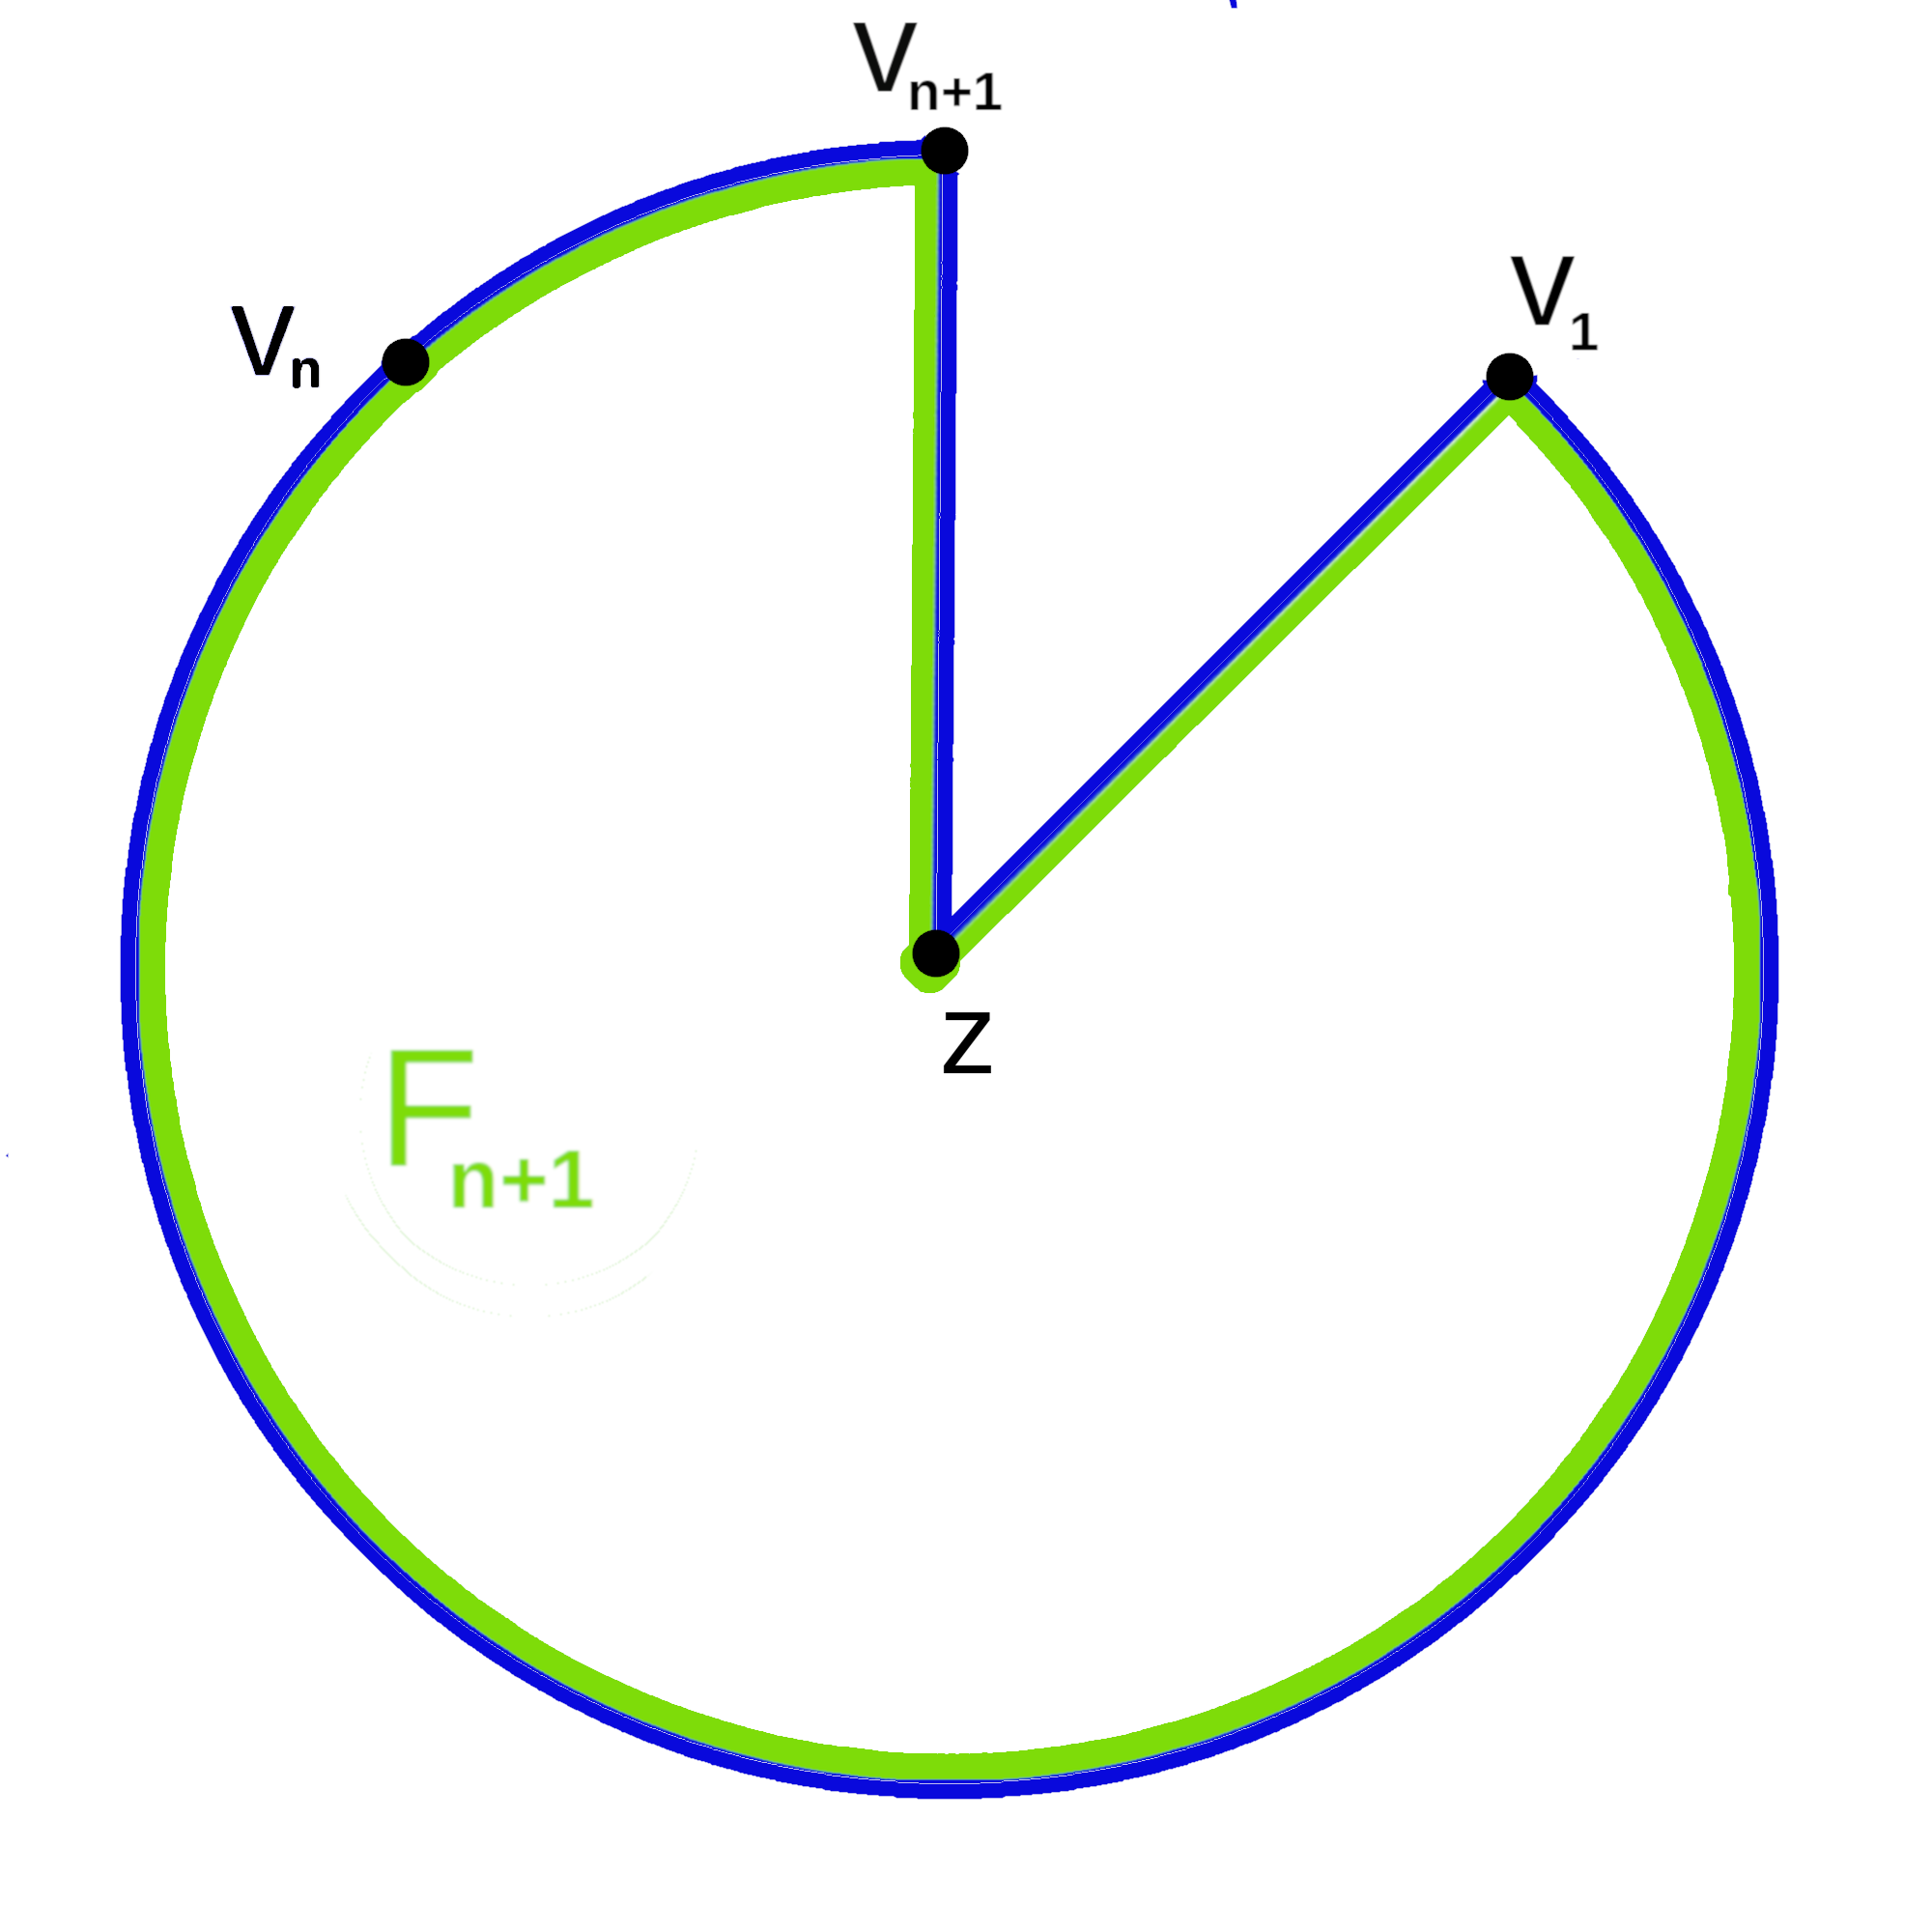
\includegraphics[width=1\textwidth]{klasse22.png}
        %\caption{In Klasse 2 sind genau die Spannbäume dieses Graphen, wobei der grün markierte Teil ein $F_{n+1}$ ist.}
        \captionof{figure}{In Klasse 2 sind genau die Spannbäume dieses Graphen, wobei der grün markierte Teil ein $F_{n+1}$ ist.}
 \label{klasse2} %caption vor label unbedingt
    \end{minipage}
%\end{figure}
\vspace{1cm}

Um zu zeigen dass die Klasse 3 genausoviele Spannbäume enthält wie $F_n$, werden wir beweisen, dass für die Anzahl der Spannbäume in Klasse 3 den gleichen rekursiven Formeln genügen, wie die von $F_n$.\\
Sei $a_n$ die Anzahl der Subgraphen von $F_n$, die aus genau zwei Komponenten bestehen, von denen eine den Knoten $z$ und die andere $v_n$ enthält.\\
Wir definieren $b_n$ als die Anzahl der Spannbäume in Klasse 3, die die Kanten $v_nv_{n+1}$ und $v_nz$ nicht enthalten.\\
Wir beweisen zuerst, dass $\mathit{k}\left(F_{n+1}\right)=2\mathit{k}\left(F_{n}\right)+a_n$ für $n\geq 2$.
Dazu nehmen wir ohne Beschränkung der Allgemeinheit an, dass $v_{n+1}$ nur zu den Knoten $v_n$ und $z$ adjazent ist. Ein Spannbaum des $F_n+1$ ist dann entweder durch hinzufügen einer der beiden Kanten $v_nv_{n+1}$ und $v_{n+1}z$ entstanden, oder durch hinzufügen beider Kanten an einen Subgraphen von $F_n$, der aus genau zwei Komponenten besteht, von denen eine den Knoten $z$ und die andere $v_n$ enthält.\\
Es gilt also $\mathit{k}\left(F_{n+1}\right)=2\mathit{k}\left(F_{n}\right)+a_n$.\\
Jetzt betrachten wir die Spannbäume aus Klasse 3.\\
Sei $M_n$ die Menge der Spannbäume von $W_{n+1}$ aus Klasse 3;\\
Nun zeigen wir, dass für $n \geq 3$ $|M_{n+1}|=2|M_n|+b_n$ ist.\\
Im folgenden betrachten wir nur $n \geq 3$. Wir erinnern uns an dieser Stelle daran, dass wir die Knoten beliebig umnummerieren können; in $M_{n+1}$ sind also die Spannbäume des Graphen aus Abbildung~\ref{mn1}.
\begin{figure}[H]
  \centering
 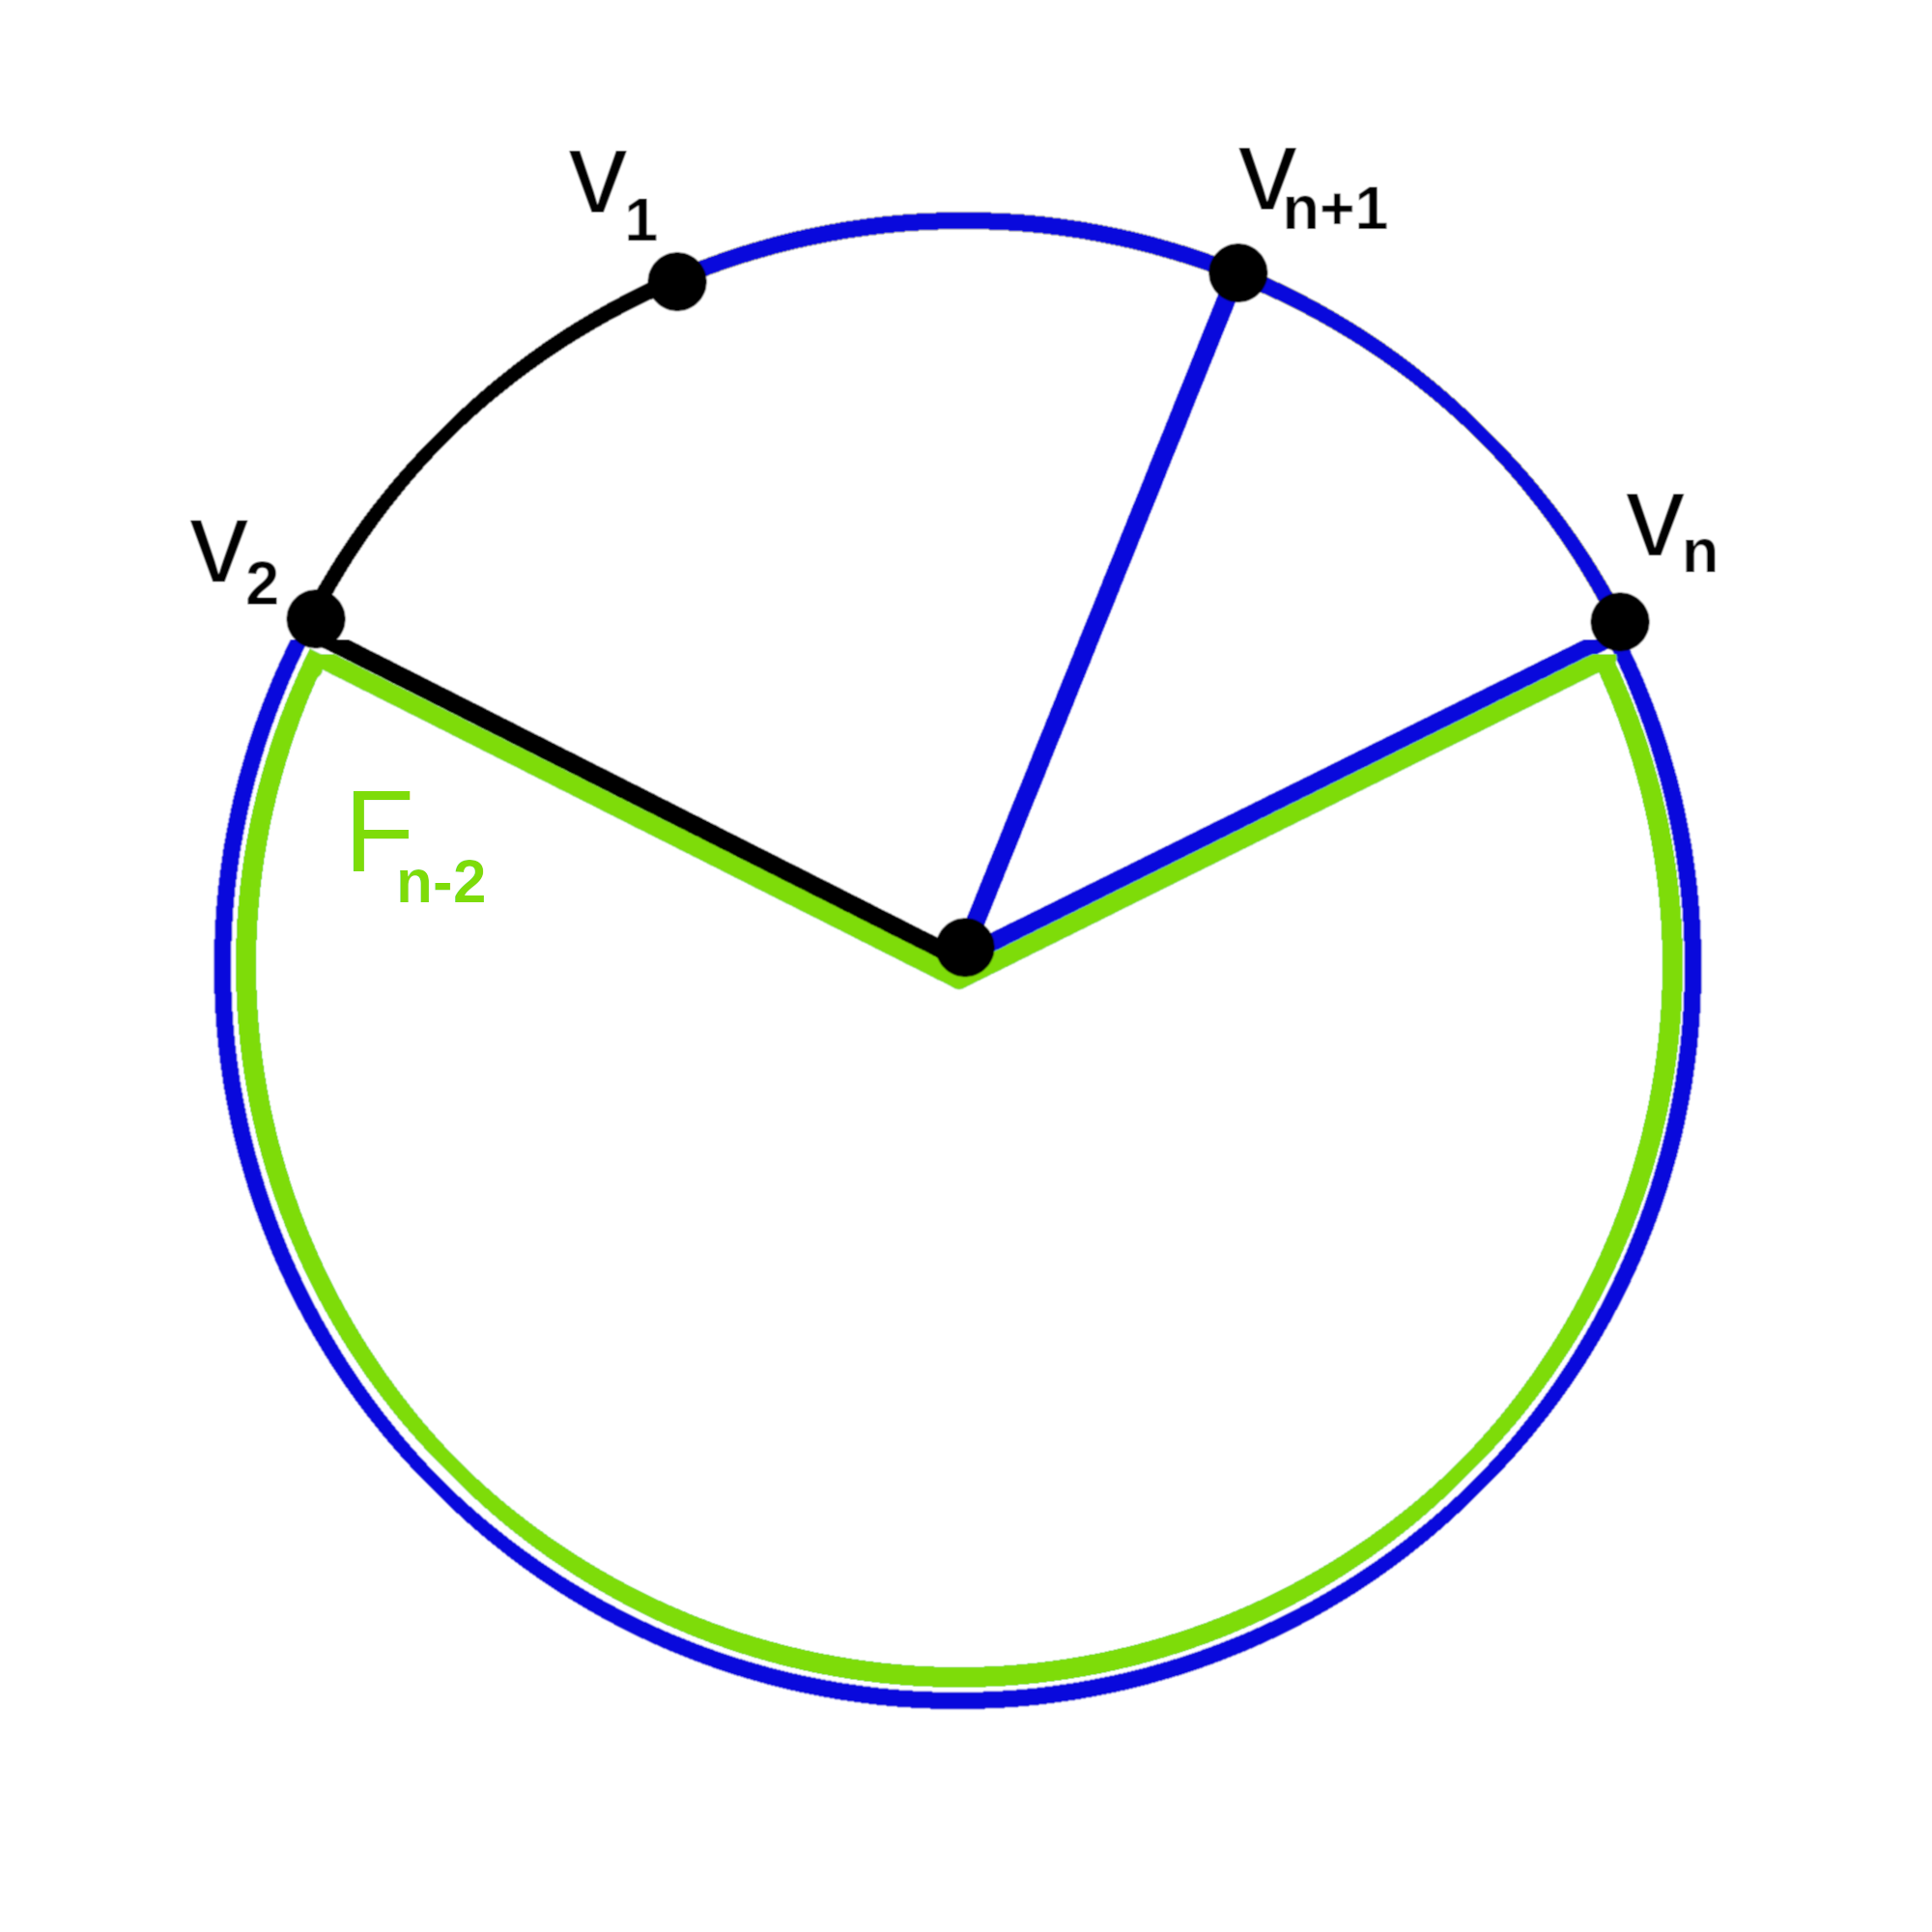
\includegraphics[width=0.5\textwidth]{mn1.png}
 \caption{}
 \label{mn1} %caption vor label unbedingt
\end{figure}
Wir unterteilen die Spannbäume davon auch in drei Klassen:\\
\par
\begingroup
\leftskip=20pt
\rightskip=20pt
\noindent
Die Erste bilden diejenigen, in denen die Kante $v_{n+1}z$ enthalten ist; Wie wir in der Abbildung~\ref{mn2} erkennen können, sind das soviele, wie in $M_n$.\\
Die Zweite besteht aus denen, die die Kante $v_nv_{n+1}$ enthalten; In Abbildung~\ref{mn3} sehen wir, dass das auch $|M_n|$ Stück sind.\\
Die Dritte beinhaltet die, die weder die Kante $v_{n+1}z$ noch die Kante $v_nv_{n+1}$ enthalten; die Anzahl davon ist nach Definition genau $b_n$.\\
\par
\endgroup
\begin{figure}[H]
    \centering
    \begin{minipage}{0.45\textwidth}
        \centering
        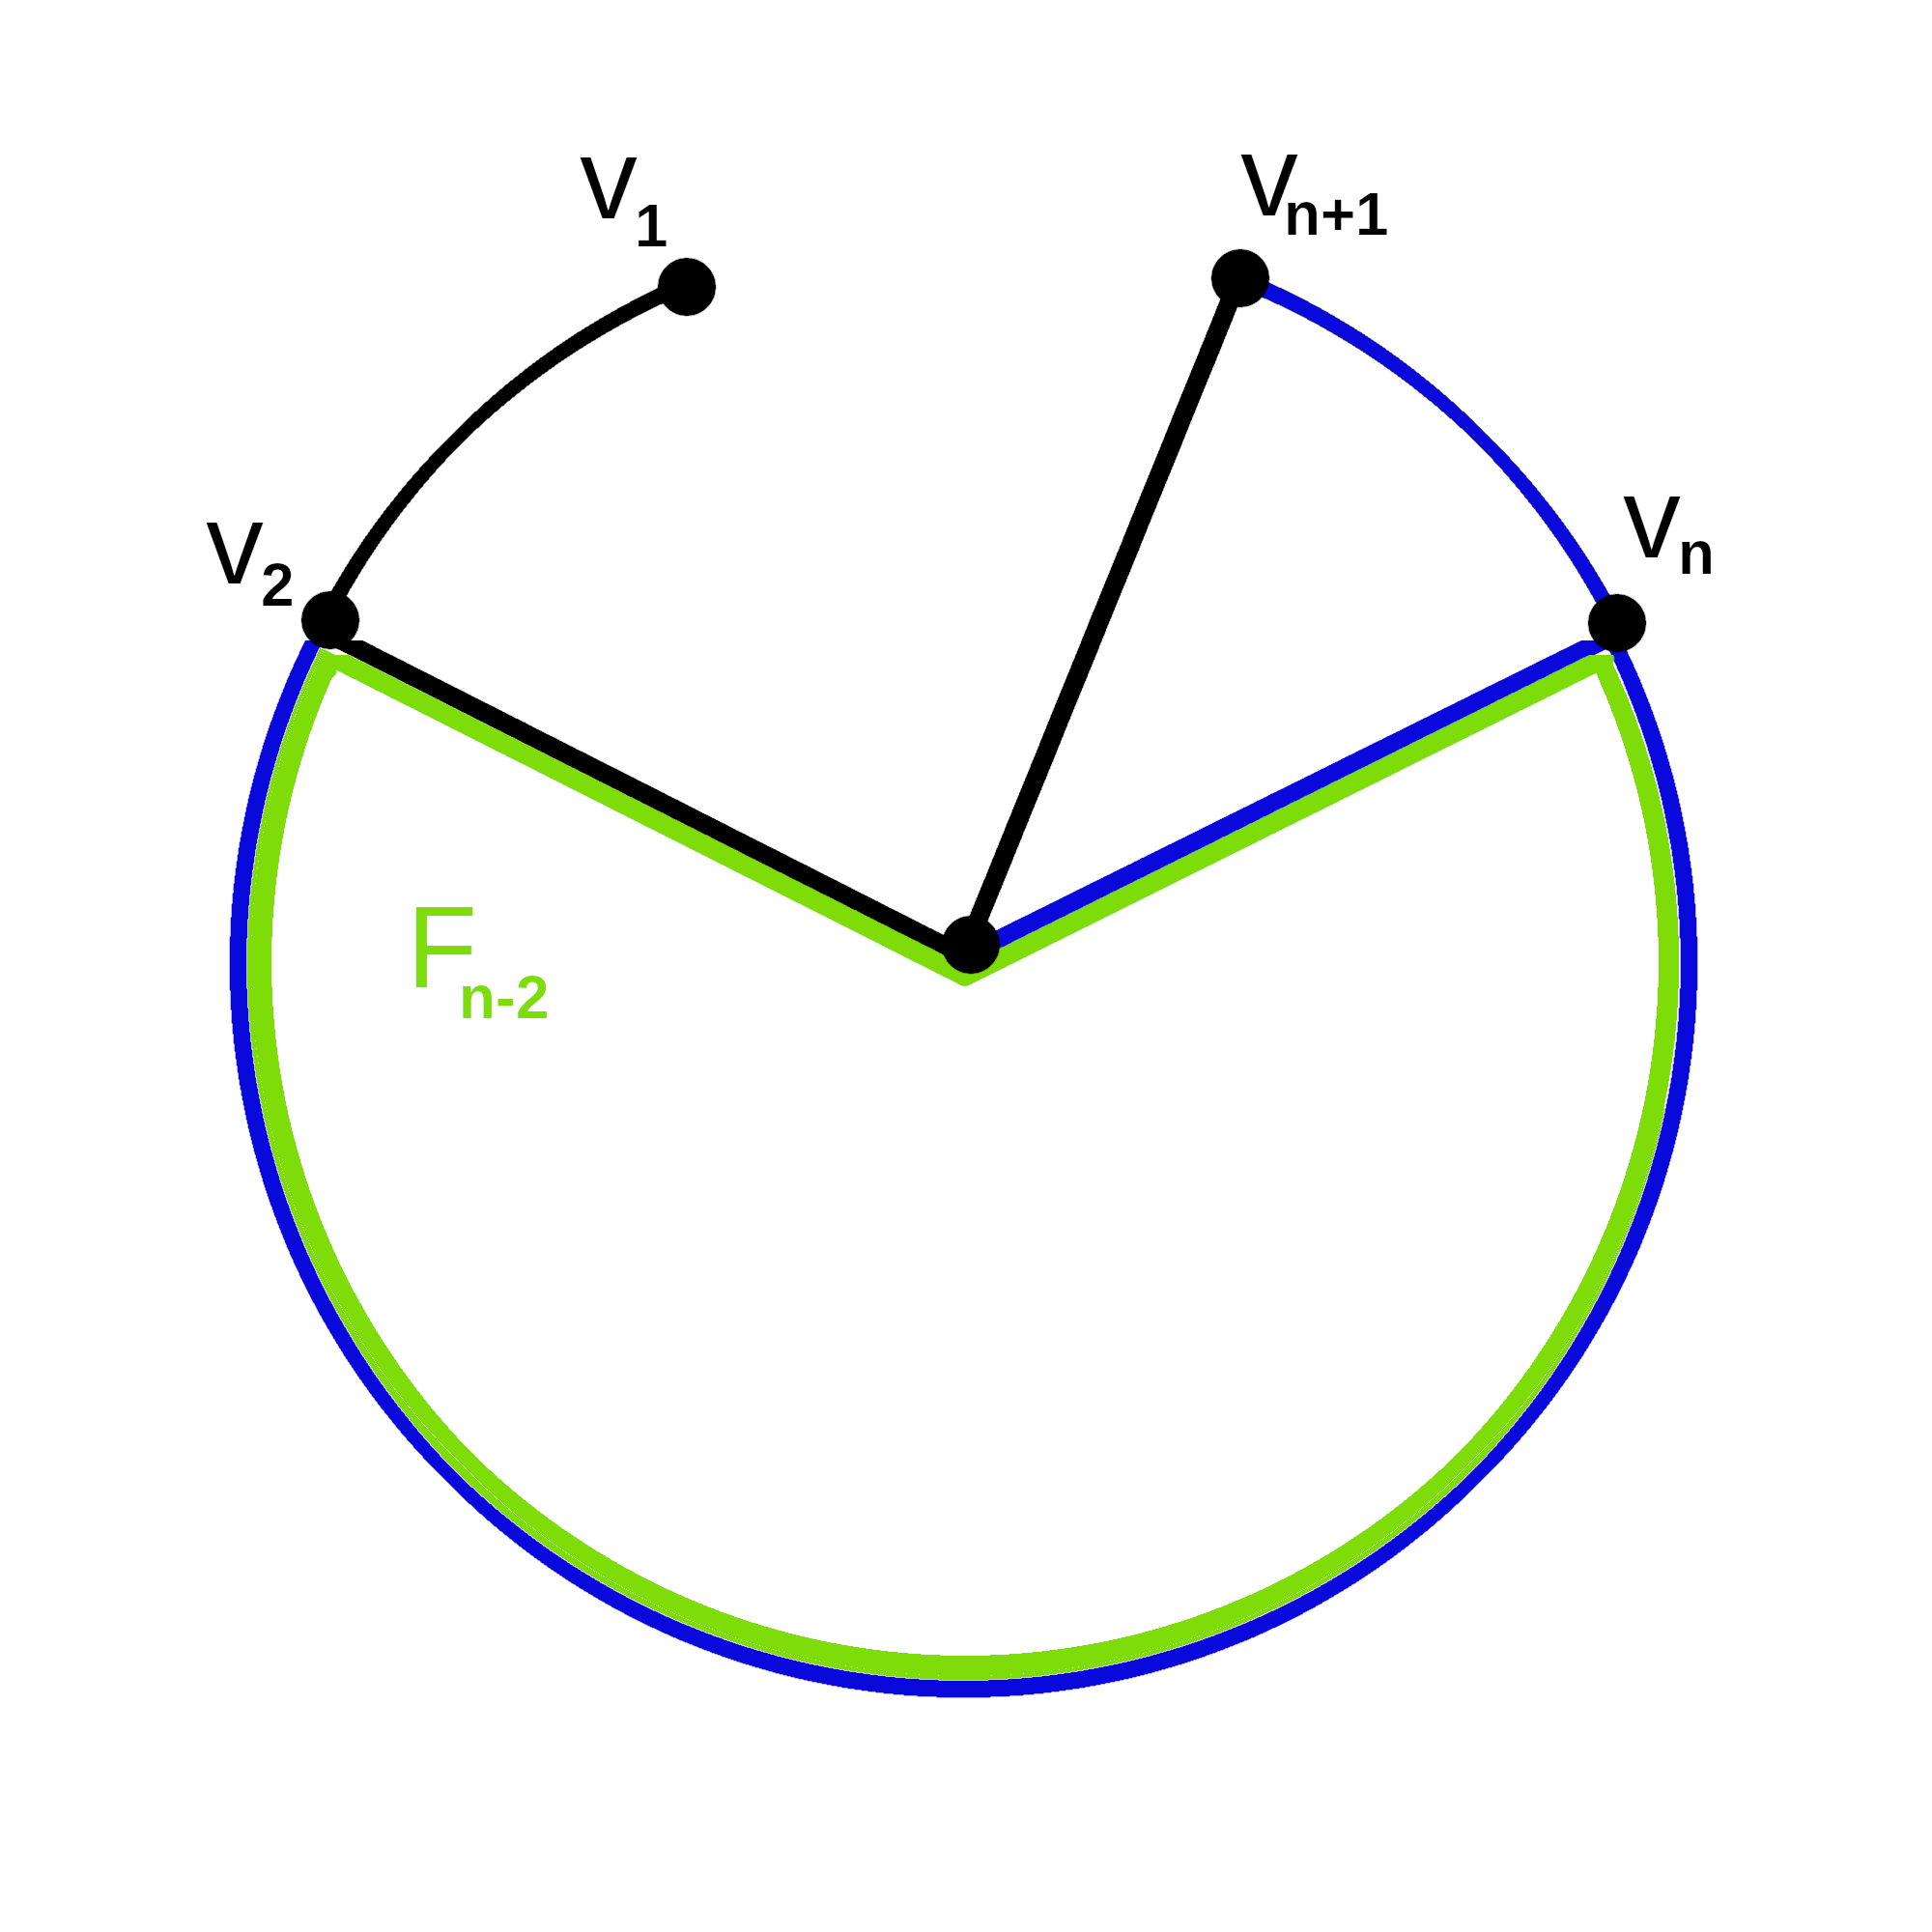
\includegraphics[width=1\textwidth]{mn2.png}
        \caption{}
 \label{mn2} %caption vor label unbedingt
    \end{minipage}\hfill
    \begin{minipage}{0.45\textwidth}
        \centering
        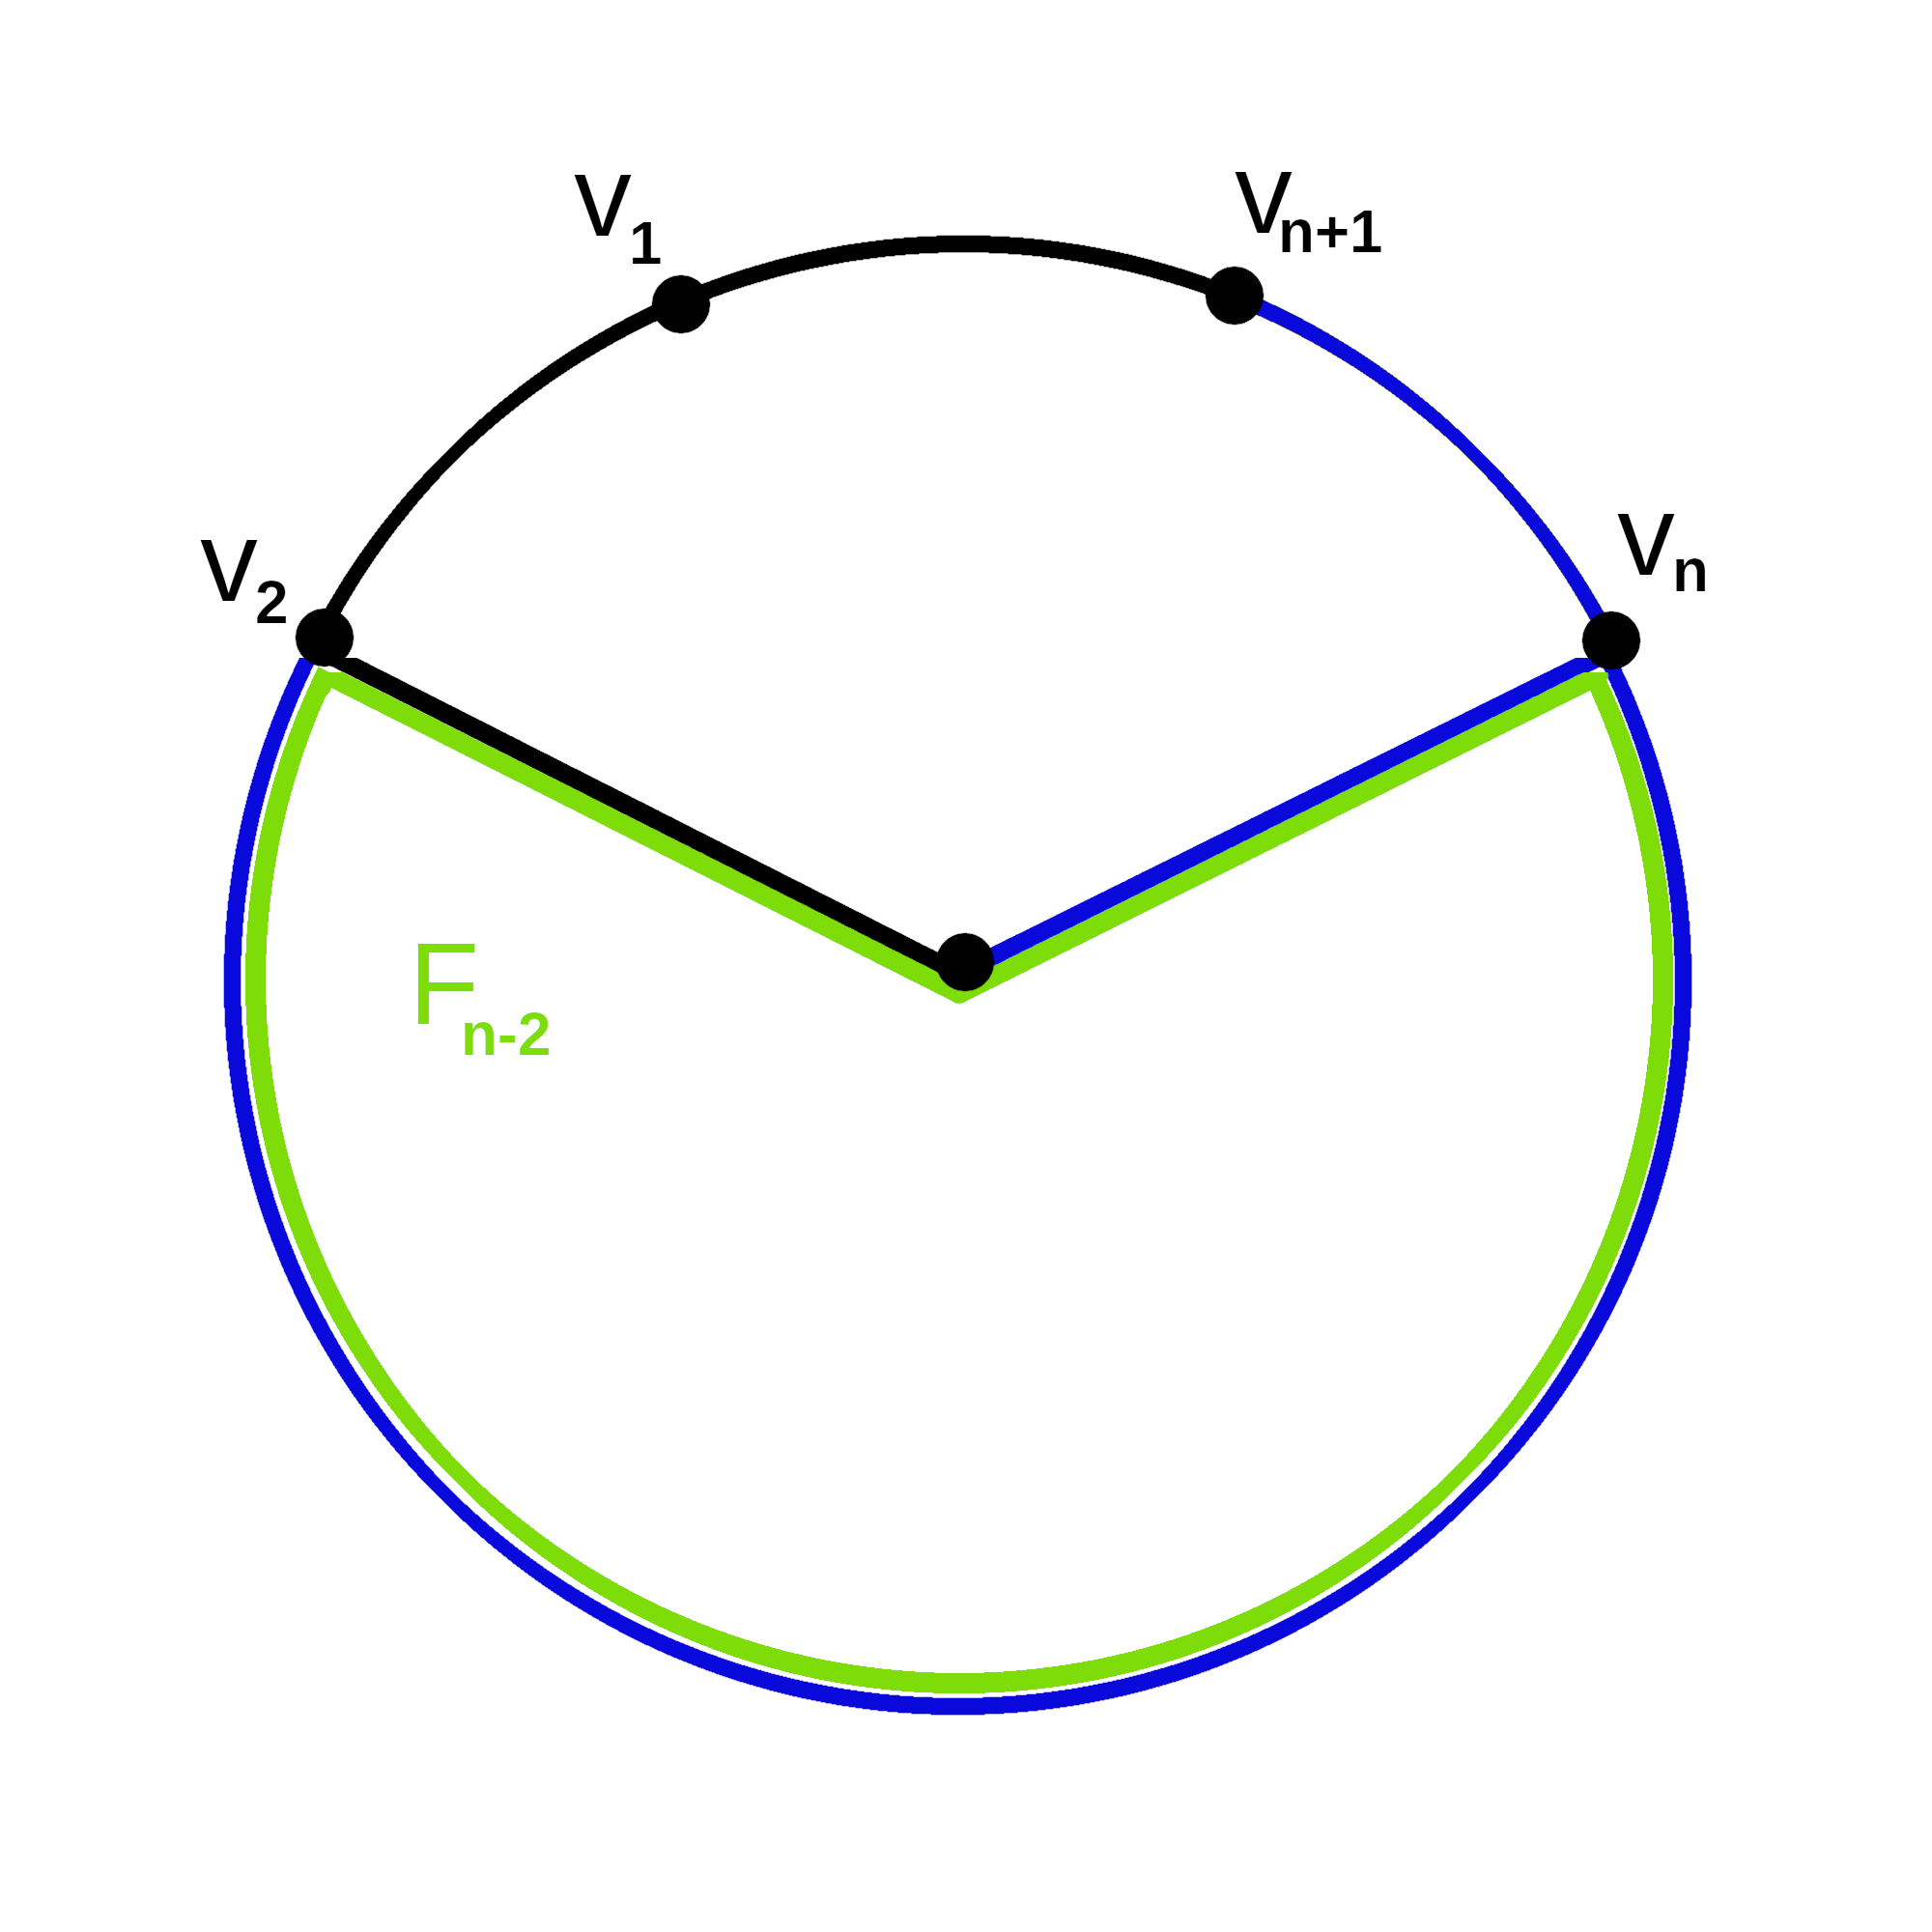
\includegraphics[width=1\textwidth]{mn3.png}
        \caption{}
 \label{mn3} %caption vor label unbedingt
    \end{minipage}
\end{figure}
Daraus schließen wir also $|M_{n+1}|=2|M_n|+b_n$ für $n\geq3$.\\
Wir sehen leicht, dass $\mathit{k}\left(F_2\right) = |M_2|$, $\mathit{k}\left(F_2\right)=|M_3|$ $a_2=b_2$ und $a_3=b_3$; daraus schließen wir, dass die Anzahl der Spannbäume in Klasse 3 gleich $\mathit{k}\left(F_{n}\right)$ ist, was wir zeigen wollten.\\
Da jeder Spannbaum von $W_{n+1}$ in genau einer der 3 Klassen ist, gilt die rekursive Beziehung
\begin{equation}
\mathit{k}\left(W_{n+1}\right) = \mathit{k}\left(F_{n+1}\right) + \mathit{k}\left(F_n\right) + \mathit{k}\left(W_n\right)
\label{eq:wrek}
\end{equation}
Wir werden nun den Beweis per Induktion über $n \in \mathbb{N}, \, n \geq 3$ vervollständigen, wobei uns natürlich zu Gute kommt, dass uns die Anzahl der Spannbäume von Fan-Graphen schon bekannt ist.\\
Für unseren Induktionsanfang sehen wir -zum Beispiel durch Anwendung von Kirchhoffs Matrix-Tree-Theorem- leicht, dass \begin{equation}
\mathit{k}\left(W_3\right) = 16 = \left(\frac{3+\sqrt{5}}{2}\right)^3+\left(\frac{3+\sqrt{5}}{2}\right)^3-2.
\end{equation}
Wir nehmen nun an, dass für ein $n \in \mathbb{N}$ die Formel 
\begin{equation}
 \mathit{k}\left(W_n\right) = \left(\frac{3+\sqrt{5}}{2}\right)^n+\left(\frac{3+\sqrt{5}}{2}\right)^n-2
\end{equation}
gilt.\\
Damit bleibt noch zu zeigen, dass
\begin{equation}
 \mathit{k}\left(W_{n+1}\right) = \left(\frac{3+\sqrt{5}}{2}\right)^{n+1}+\left(\frac{3+\sqrt{5}}{2}\right)^{n+1}-2.
\end{equation}
Das werden wir nun einfach ausrechnen.
Nachdem wir im vorherigen Kapitel herausgefunden haben, wieviele Spannbäume Fan-Graphen haben, setzen wir das und unsere Induktionsannahme in die Gleichung (\ref{eq:wrek}) ein, und erhalten:\\
\begin{equation}
\begin{aligned}
\mathit{k}\left(W_{n+1}\right) ={} & \frac{\left(3+\sqrt{5}\right)^{n+1}-\left(3-\sqrt{5}\right)^{n+1}}{2^{n+1}\sqrt{5}} + \frac{\left(3+\sqrt{5}\right)^{n}-\left(3-\sqrt{5}\right)^{n}}{2^{n}\sqrt{5}}\\
& + \left(\frac{3+\sqrt{5}}{2}\right)^n+\left(\frac{3-\sqrt{5}}{2}\right)^n-2
\end{aligned}
\end{equation}
Wir bringen fast alles auf einen Nenner, sortieren die Terme und bekommen
\begin{equation}
\begin{aligned}
\mathit{k}\left(W_{n+1}\right) = {}  & \frac{\left(3+\sqrt{5}+2+2\sqrt{5}\right)\left(3+\sqrt{5}\right)^{n}}{2^{n+1}\sqrt{5}} \\%% {} steht da nur, weils hin muss, wegen dem =
                        & -\frac{\left(3+\sqrt{5}+2-2\sqrt{5}\right)\left(3-\sqrt{5}\right)^{n}}{2^{n+1}\sqrt{5}}-2 
\end{aligned}
\end{equation}
\todo[inline]{evtl. zusammengehörige Terme evtl. farbig markieren}
Ausrechnen führt uns zu\\
\begin{equation}
\mathit{k}\left(W_{n+1}\right) = \left(\frac{3+\sqrt{5}}{2}\right)^{n+1}+\left(\frac{3+\sqrt{5}}{2}\right)^{n+1}-2
\end{equation}
Damit ist unser Induktionsbeweis abgeschlossen und wir haben gezeigt, dass unser Satz \ref{wn} über die Anzahl der Spannbäume in einem Rad gilt.
\begin{flushright} $\Box$ \end{flushright} 
